\documentclass[border=6pt]{standalone}
\usepackage{helvet}
\renewcommand{\familydefault}{\sfdefault}
\usepackage{amsmath}
\usepackage{tikz}
\usetikzlibrary{shapes.geometric, arrows.meta, positioning, calc, fit, backgrounds}

\begin{document}
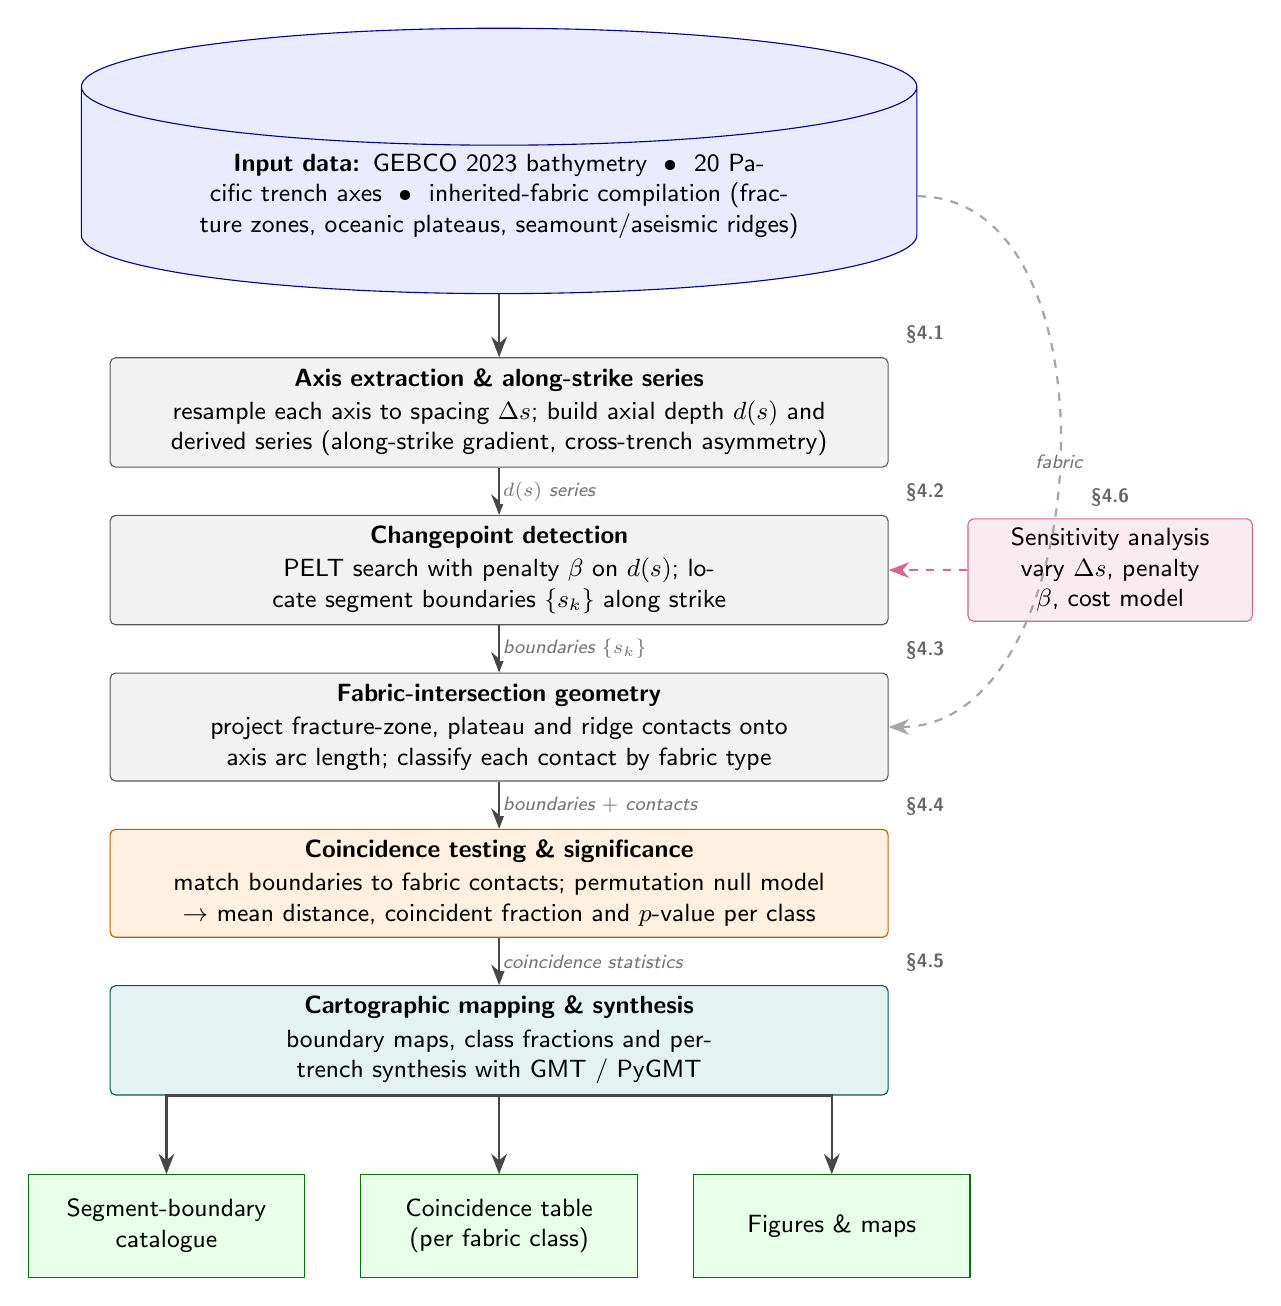
\begin{tikzpicture}[
  font=\small,
  >={Stealth[length=2.6mm,width=2mm]},
  every node/.style={transform shape},
  data/.style={cylinder, shape border rotate=90, aspect=0.14, draw=blue!55!black,
               fill=blue!8, text width=104mm, align=center, minimum height=13mm,
               inner sep=3pt},
  proc/.style={rounded corners=2pt, draw=black!65, fill=black!5, text width=96mm,
               align=center, minimum height=12mm, inner sep=4pt},
  stat/.style={rounded corners=2pt, draw=orange!75!black, fill=orange!12,
               text width=96mm, align=center, minimum height=12mm, inner sep=4pt},
  mapb/.style={rounded corners=2pt, draw=teal!70!black, fill=teal!10,
               text width=96mm, align=center, minimum height=12mm, inner sep=4pt},
  outp/.style={draw=green!45!black, fill=green!9, text width=33mm, align=center,
               minimum height=13mm, inner sep=3pt},
  side/.style={rounded corners=2pt, draw=purple!60, fill=purple!8, text width=34mm,
               align=center, minimum height=13mm, inner sep=3pt},
  tag/.style={font=\scriptsize\bfseries, text=black!60},
  elab/.style={font=\scriptsize\itshape, text=black!55, fill=white, inner sep=1pt},
  arr/.style={->, thick, black!72},
  darr/.style={->, thick, purple!60, dashed},
  node distance=6mm
]

\node[data] (in) {\textbf{Input data:} GEBCO 2023 bathymetry \ \textbullet\ \
  20 Pacific trench axes \ \textbullet\ \ inherited-fabric compilation
  (fracture zones, oceanic plateaus, seamount/aseismic ridges)};

\node[proc, below=8mm of in] (p1)
  {\textbf{Axis extraction \& along-strike series}\\[1pt]
   resample each axis to spacing $\Delta s$; build axial depth $d(s)$ and
   derived series (along-strike gradient, cross-trench asymmetry)};
\node[tag, above right=0.5mm and 1mm of p1.north east] {\S4.1};

\node[proc, below=of p1] (p2)
  {\textbf{Changepoint detection}\\[1pt]
   PELT search with penalty $\beta$ on $d(s)$; locate segment boundaries
   $\{s_k\}$ along strike};
\node[tag, above right=0.5mm and 1mm of p2.north east] {\S4.2};

\node[proc, below=of p2] (p3)
  {\textbf{Fabric-intersection geometry}\\[1pt]
   project fracture-zone, plateau and ridge contacts onto axis arc length;
   classify each contact by fabric type};
\node[tag, above right=0.5mm and 1mm of p3.north east] {\S4.3};

\node[stat, below=of p3] (p4)
  {\textbf{Coincidence testing \& significance}\\[1pt]
   match boundaries to fabric contacts; permutation null model $\rightarrow$
   mean distance, coincident fraction and $p$-value per class};
\node[tag, above right=0.5mm and 1mm of p4.north east] {\S4.4};

\node[mapb, below=of p4] (p5)
  {\textbf{Cartographic mapping \& synthesis}\\[1pt]
   boundary maps, class fractions and per-trench synthesis with GMT / PyGMT};
\node[tag, above right=0.5mm and 1mm of p5.north east] {\S4.5};

\node[outp, below=10mm of p5] (o2) {Coincidence table\\(per fabric class)};
\node[outp, left=7mm of o2] (o1) {Segment-boundary catalogue};
\node[outp, right=7mm of o2] (o3) {Figures \& maps};

\node[side, right=10mm of p2] (sens)
  {Sensitivity analysis\\ vary $\Delta s$, penalty $\beta$, cost model};
\node[tag, above=0.3mm of sens.north] {\S4.6};

\draw[arr] (in) -- (p1);
\draw[arr] (p1) -- (p2) node[elab, midway, right] {$d(s)$ series};
\draw[arr] (p2) -- (p3) node[elab, midway, right] {boundaries $\{s_k\}$};
\draw[arr] (p3) -- (p4) node[elab, midway, right] {boundaries $+$ contacts};
\draw[arr] (p4) -- (p5) node[elab, midway, right] {coincidence statistics};
\draw[arr] (p5.south) -- (o2.north);
\draw[arr] (p5.south) -| (o1.north);
\draw[arr] (p5.south) -| (o3.north);
\draw[darr] (sens.west) -- (p2.east);

\draw[darr, black!35] (in.east) to[out=0,in=0]
      node[elab, pos=0.5]{fabric} (p3.east);

\end{tikzpicture}
\end{document}
